% !TEX root = ../master.tex

\newcommand{\labelof}[1]{\underline{#1}}
\newcommand{\dlmactsfor}{\dlmc{if\_acts\_for}}
\newcommand{\dlmdeclassify}{\dlmc{declassify}}
\newcommand{\dlmpc}{$\underline{pc}$}
\newcommand{\mathcomment}[1]{\color{green!50!black}{#1}}
\newcommand{\ceil}[1]{\lceil#1\rceil}

\chapter{The Decentralized Label Model}\label{dlm}
The Decentralized Label Model \cite{myers1997, myers1998, myers2000} is a model for ensuring information flow control in a system.
This is done by annotating source code with security policies, in the form of labels attached to data-holding constructs.
This chapter will present the necessary information needed to understand the implementation presented in \cref{ctif}.
The descriptions and definitions in this section are based on \cite{myers1997, myers1998, myers2000}.
Throughout the examples, we will use the same grammar as that used by our implementation.

In this presentation of DLM some details have been left out.
These details are related to run-time concepts, such as \emph{principal hierarchy} and \emph{authority}.
Our focus will be on the concepts needed for compile-time checking.
\mikkel{Reminder about principal hierarchies}\rene{Vigtigt!}

Finally, in \cref{dlm:constraints,dlm:inferring_labels} we will present our own formalizations related to the concept of \emph{label inferrence}, which is briefly introduced in \cite{myers1997}.
We will use these formalizations as a base in order to define the label inferrence algorithm, which is an essential part of our implementation.

\section{Labels and Policies}\label{dlm:policies}
Throughout a program, values are declared, initialized, and assigned to variables and other value-holders.
Value-holders are collectively known as \emph{slots}, which cover constructs such as variables, structs, and other storage locations.
In order to ensure that a certain assignment is legal, such that no information is unintentionally leaked, we assign \emph{labels} to slots so that their ``security'' can be compared.
This way we can ensure that an assignment is only legal in the cases where higher-security values aren't assigned to lower-security slots.
The same concept applies to more complex language constructs, such as functions (and their return values).
\mikkel{Function labels? Mangler vi en oversigt over hvor det er muligt at deklarere labels?}

Each slot is associated with a label, that describes how the data in the slot can be handled.
We denote the label of slot $s$ as $\underline{s}$.
Referring to labels in this fashion serves the same purpose as letters in algebra; it allows for handling labels without knowledge about their actual value.

For a given label it is possible to define both read (\emph{privacy}) and write (\emph{integrity}) policies.
The first represents information flow out of a system and the latter information flow into a system.
In this report only read policies will be considered.
Due to the relation between the two types of policies, we note that write policies can be ensured in a fashion similar to read policies.
Because of this we choose to simplify the scope of the report such that it only discusses read policies.

\myparagraph{Principals}
In the following, we employ the concept of \emph{principals}.
A principal (or \emph{subject}, \emph{agent}) is an entity in a system that represents some interest.
In short, principals represent real-world users or the authority under which a program/system runs.

In the following we make use of the special set of principals; $*$.
This set contains all the principals in a system.

\myparagraph{Labels}
A label can be described as a set of policies, where a policy consists of an owner principal $o$ and a set of reader principals $r_1, r_2, \dots, r_n$.
Formally we provide the following, equivalent definition:
\begin{definition}{Labels}\label{dlm:def:label}
A label $L$ is a set of owners $owners(L)$, and a function $readers(L, o)$ that retrieves the set of reader principals that $o$ allows to read.
Note that given this definition we have that $$o \notin owners(L) \Rightarrow readers(L, o) = *$$
\end{definition}

Owners are allowed to change their own policies within a label.
We describe how this is done in \cref{dlm:auth_and_declass}.
If an owner is not part of its own policies reader set, that owner is not allowed to read from the slot associated with the label.
He is however still allowed to change his policy.

\myparagraph{The effective reader set}
To ensure that the policies of all owners in a label are enforced, only readers that all owners ``agree'' can read from the slot associated with the label.
This is known as the \emph{effective reader set}, which is the intersection of \emph{all} reader sets of a label:
\begin{definition}{The effective reader set}\label{dlm:def:effectivereaders}
  The reader set of a label $L$ is the set of readers that are in the reader set of all owners:
  $$readers(L) = \bigcap_{o \in *} readers(L, o)$$
\end{definition}

\begin{example}{A label with two policies}\label{dlm:ex:simple_label}
  Below is an example of a label with two policies using the notation from above;
  $$L_1 = \{o1 \rightarrow r1, r2; o2 \rightarrow r2, r3\}$$

  The owner set of the label is $owners(L_1) = \{o1, o2\}$, and its reader sets are $readers(L_1, o1) = \{r1, r2\}, readers(L_1, o2) = \{r2, r3\}$.
  By intersecting the reader sets of the label we get the effective reader set.
  In practice we can disregard the reader set of labels that are not owners.
  Thus the effective reader set is
  $$readers(L_1) = \{r1,r2\} \cap \{r2, r3\} = \{r2\}$$
\end{example}

\section{Security class lattice}
A set of DLM labels can be seen as a \emph{security class lattice} \cite[pp. 6-7]{myers1997}.
A lattice is a partially ordered set, for which each pair of elements in the set have a unique least upper bound (the join/$\sqcup$ of the labels) and a greatest lower bound (the meet/$\sqcap$ of the labels).
In the case of DLM, the lattice is the set of all labels and it is ordered by how restrictive the labels are.

A label without owners effectively has no restrictions on the data it protects.
As such it is the lower bound $\bot$ of the lattice.
Likewise the label that has all owners in a system (as defined in \cref{dlm:def:label}), but no readers allowed by either of the owners, is the most restrictive label.
This is the upper bound $\top$ of the lattice.

With these we have a bounded lattice as illustrated by \cref{dlm:lattice_fig}.
In the following sections we define the properties of this security lattice.
These will match the description of the lattice bounds given above.

\begin{figure}
  \begin{center}
  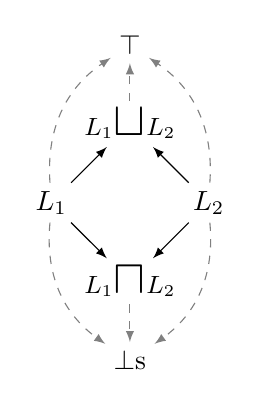
\begin{tikzpicture}[inner sep=1mm, >=latex]
    \node (l1) at (-1,0) {$L_1$};
    \node (l2) at (1,0) {$L_2$};

    \node (meet) at (0,-1) {\small $L_1$ {\LARGE $\! \sqcap \!$} $L_2$};
    \node (bot) at (0,-2) {$\bot$s};

    \node (join) at (0,1) {\small $L_1$ {\LARGE $\! \sqcup \!$} $L_2$};
    \node (top) at (0,2) {$\top$};

    \draw[->] (l1) edge (join);
    \draw[->] (l2) edge (join);
    \draw[->] (l1) edge (meet);
    \draw[->] (l2) edge (meet);

    \draw[->, dashed, gray] (l1) edge [bend left] (top);
    \draw[->, dashed, gray] (join) edge (top);
    \draw[->, dashed, gray] (l2) edge [bend right] (top);

    \draw[->, dashed, gray] (l1) edge [bend right] (bot);
    \draw[->, dashed, gray] (meet) edge (bot);
    \draw[->, dashed, gray] (l2) edge [bend left] (bot);
  \end{tikzpicture}
  \caption{Abstraction of security lattice}
  \label{dlm:lattice_fig}
  \end{center}
\end{figure}

\subsection{Composite labels}
We can construct composite labels by either joining or meeting two labels.
A composite label $L_1 \sqcup L_2$ or $L_1 \sqcap L_2$ represents nodes in a composite label structure.
To employ these labels similarly to the previously defined labels, we define the owner and reader sets of the composite labels:

\begin{definition}{Label Join}\label{dlm:def:join}
The join operation is denoted by the operator $\sqcup$ and represents the least restrictive label that is as restrictive as either operand:
  \begin{align*}
    owners(L_1 \sqcup L_2) &= owners(L_1) \cup owners(L_2) \\
    readers(L_1 \sqcup L_2, o) &= readers(L_1, o) \cap readers(L_2, o)
  \end{align*}
\end{definition}
\begin{definition}{Label Meet}\label{dlm:def:meet}
The meet operation is denoted by the operator $\sqcap$ and represents the most restrictive label that is no more restrictive than either operand:
  \begin{align*}
    owners(L_1 \sqcap L_2) &= owners(L_1) \cap owners(L_2) \\
    readers(L_1 \sqcap L_2, o) &= readers(L_1, o) \cup readers(L_2, o)
  \end{align*}
\end{definition}

Label composition is an integral part of DLM.
Label joins allows for label evaluation of expressions, as described in \cref{extraction} and provides the means for representing implicit flows via scope blocks, as described in \cref{dlm:implicit_flows}.
Additionally when inferring labels, the meet operation allows us to infer the most restrictive label that agrees with the preexisting labels.

\subsection{Label comparison}\label{dlm:comparison}
As mentioned above, labels provide restrictions on how data can flow to and from slots that the labels ``protect''.
In order to check that security policies are enforced throughout a program, we need to be able to compare how restrictive labels are.
To do this we introduce the ``at most as restrictive as''-relation ($\sqsubseteq$) from \cite{myers1997}.

\begin{definition}{Label Restrictiveness}\label{dlm:def:restrict}
  Label $L_1$ is at most as restrictive as label $L_2$ ($L_1 \sqsubseteq L_2$) if it (1) does not have more owners and (2) each owner does not have a smaller reader set:
  \begin{align*}
    & \text{(1) } owners(L_1) \subseteq owners(L_2) \text{ and} \\
    & \text{(2) } \forall o \in owners(L_1) . readers(L_1, o) \supseteq readers(L_2, o)
  \end{align*}
\end{definition}

We can employ this definition to determine if two labels are equal:
If $L_1 \sqsubseteq L_2$ and $L_2 \sqsubseteq L_1$ then we must have that $L_1 = L_2$.
Additionally we note that given \cref{dlm:def:join,dlm:def:restrict} we note that $L_1 \sqcup L_2 \sqsubseteq L_3$ is equivalent to $L_1 \sqsubseteq L_3 \wedge L_2 \sqsubseteq L_3$.
This provides a simplified means for comparing composite label-structures.

\section{Channels}\label{dlm:channels}
Throughout a system data can enter and leave, before- and afterwhich labels cannot be enforced.
The entry points for data entering and leaving can therefore be seen as crucial endpoints, where we want to do additional checking to ensure we are not unintentionally leaking.
This is done through \emph{channels}, specifically \emph{input channels} and \emph{output channels}.
However, input channels are not special and simply apply the label of the channel to the inputted data.

\myparagraph{Output channels}
On the other hand, output channels are especially crucial in that it is an endpoint where we will intentionally ``leak'' data, and afterwhich we are not able to control the further flow of this data.
Intuitively, an output channel represents data going outside the system, e.g. through a physical printer, console output, or web request.

Output channels therefore differ in the way that the ``security'' is compared.
Output channels need only declare a list of readers, that represent the principals that have access to the endpoint.
We then need to compare this reader list to the effective reader set of the label for the data to be outputted.
Any reader declared by the output channel must be in the effective reader set for the label of the outputted data, to ensure that we do not output data to a channel where the principals aren't allowed to read it.

\section{Implicit flows}\label{dlm:implicit_flows}
When assigning a value to a slot, possibly from another slot, it is an explicit flow.
In addition to explicit flows, it is also possible to have implicit flows throughout a program, due to conditional control structures (such as loops).
For whatever assignments we would do inside a block (or within a deeper block hierarchy) we need to take the predicates of these blocks into consideration.
This is done by adding the concept of \emph{program counter labels}, denoted \dlmpc.
For each scope we will have an implicit \dlmpc, depending on the surrounding predicates' labels.

\begin{example}{Implicit leak}\label{dlm:ex:implicit_leak}
  Consider the following program (each line commented with the current \dlmpc):
  \begin{lstlisting}[style=dlmc]
int {{a->z,y}} val = 0;   // $\mathcomment{\bot}$
int {{a->y}} cond = 1;    // $\mathcomment{\bot}$
if (cond) {
  val++;                  // $\mathcomment{\bot \sqcup \{a \rightarrow y\}}$
}
return val;               // $\mathcomment{\bot}$
  \end{lstlisting}
  In this example we would have an implicit leak of \dlmc{cond}, by way of \dlmc{val}.
  This is due to the assignment of \dlmc{val} inside of the \dlmc{if}-statement, as \dlmpc~ is increased to the join of the outer scope ($\bot$) and the label of the scope's predicate (\labelof{\dlmc{cond}}).
  For this program to pass \thetool, we would have to add a more strict policy to \dlmc{val}, so that it could match the policy of \dlmc{cond}.
\end{example}

\section{Authority and declassification}\label{dlm:auth_and_declass}
In order to avoid mishaps by setting certain policies too lax, so that certain flows are permitted, we can temporarily set some policies to be more strict, and then only relax (\emph{declassify}) them when we really need to.
In order to do this, the concept of \emph{authority} is introduced.

At any point during execution of a program, there will be a \emph{true authority}, which is the maximal authority by which the program can carry out operations.
Whenever we call a function, we can do this with a certain authority, corresponding to running that method with the authority of a specific principal or principals.
However, in order to take advantage of this given authority, we need to explicitly claim it.
This is done by using the \emph{if acts for} construction\footnote{We use the syntax: \dlmc{-->? p1, p2 \{ /*statements*/ \}} -- more about this in \cref{ctif:informal:ifactsfor_declassify}).}, which takes as an argument one or more principals for which we want to obtain authority to carry out statements in the block.
Only after calling this function will we obtain the \emph{effective authority} to act for the principals, enabling us to carry out the statements within the  block that would normally only be permissible for the principals themselves.

If the check fails, the statements block is not executed.
If the check passed, the statements will be executed under the the newly established authority, e.g. for a principal $p$.
With $p$ in the effective authority we can perform declassification -- deliberately and explicitly relaxing the security policies in which $p$ is owner.
This is done by using the \emph{declassify} construction\footnote{We use the syntax: \dlmc{<|v, l|>} -- more about this in \cref{ctif:informal:ifactsfor_declassify}).}, with a slot $v$ and a new label $l$ as arguments, returning the value $v$ relabeled to $l$.
The relabeling by declassification rule (the inference rule) is defined as follows:

\begin{definition}{Relabeling by declassification}
  Let $P$ denote the set of principals in the current authority, then
  \[
  \frac
  {
    \splitfrac
    {
      L_A = \mathlarger\sqcupl_{p \in P} \{p \rightarrow \emptyset \}
    }
    {
      L_1 \sqsubseteq L_2 \sqcup L_A
    }
  }
  {
    L_1 \text{ may be declassified to } L_2
  }
  \]
\end{definition}

The combination of these two concepts, \emph{if acts for} and \emph{declassify}, is especially useful when we have sensitive inputs to a method and want to carry out our calculations without the fear of neither explicit or implicit leakage.
This way we can keep our strict policies throughout the calculations of the method and only relax the label once we want to return the result.

\begin{example}{Temporarily restricting a label}
  Building on \cref{dlm:ex:implicit_leak}, we can set the label for \dlmc{val} to match that of \dlmc{cond}, and then only relax that label when we need to return \dlmc{val}, ensuring that we have the ability to do so:
  \begin{lstlisting}[style=dlmc]
int {{a->y}} val = 0;
int {{a->y}} cond = 1;
if (cond) {
  val++;
}
-->? a {
  return <|x, {{a->y,z}}|>;
}
return -1;
  \end{lstlisting}
  While we still leak some information about \dlmc{cond}, we now do it explicitly.
\end{example}

\section{Label constraints}\label{dlm:constraints}
Using the concept of labels as described in the above sections, code can be annotated to express what type of information flow is permissible.
By examining all points in code where information flows it can then be determined if these information flows are valid.
The validity of an information flow is expressed as a constraint on the form $L_1 \sqsubseteq L_2$, as described in \cref{dlm:def:restrict}.

When information flows from one point $A$ to another $B$, it is required that $B$ is allowed to read the same information as $A$.
Thus we can, in general, represent such an information flow as $\labelof{A} \sqsubseteq \labelof{B}$.
This represents that access to the information known at point $A$ is no more restrictive than access to that of point $B$.
An example of such an information flow is the assignment of a value to a variable:

$$var := expression$$

From this simple example it is clear that information flows from the expression to the variable and thus a constraint for this example would be $\labelof{expression} \sqsubseteq \labelof{var}$.
Though as we described in \cref{dlm:implicit_flows} information can also flow implicitly, and because of that we must include all available information in the flow constraint.
The currently available information is represented as the program counter $\labelof{pc}$ and must be included on the left side of the constraint, to produce:

$$\labelof{expression} \sqcup \labelof{pc} \sqsubseteq \labelof{var}$$

This expansion of constraints captures that information assigned to $var$ could contain information about the values on which the current program counter is based.
Implicit flows will thus be considered similarly to any other constraints.

\myparagraph{Extracting constraints}
The above example illustrates the concept of information flow as described by a constraint.
The information flow of a program can be describe by a number of constraints.
Checking that each constraint is valid using \cref{dlm:def:restrict} will ensure that the information flow of the entire program is valid, given the declared labels.
In \cite{myers1997, myers1998, myers2000} an informal description of which constraints a program is associated with is provided.
In \cref{extraction} we provide a formalized approach to extracting constraints from label declarations.

Below is a simple example of the how labels and constraints are extracted from source code.
The example does not consider some of the complexities that arise from checking a complete function (or set of functions), but merely serves to provide a simple example of what checking constraints entails.

\begin{example}{Declaration and assignment}\label{dlm:ex:extract}
  Two variable declarations with associated labels and an assignment operation.

  \begin{lstlisting}[style=dlmc]
int {{a->y, x}} val = 5;  // $\mathcomment{\{a \rightarrow y, x\}}$, $\mathcomment{\labelof{5} \sqsubseteq \labelof{val}}$
int {{a->y}} res;         // $\mathcomment{\{a \rightarrow y\}}$

res = val;                // $\mathcomment{\labelof{val} \sqsubseteq \labelof{res}}$
  \end{lstlisting}

  As described above, the assignment operation introduces a constraint that must be checked for the information flow to be valid.
  Additionally the declaration of the \dlmc{val} variable includes an assignment operation.
  Because of this we have an additional, yet trivial, constraint for the declaration.
  Thus we have the following constraints for the above code and know that the information flow in the code is valid.
  $$\labelof{5} \sqsubseteq \labelof{val} \equiv \bot \sqsubseteq \{a \rightarrow y, x\}$$
  $$\labelof{val} \sqsubseteq \labelof{res} \equiv \{a \rightarrow y, x\} \sqsubseteq \{a \rightarrow y\}$$
\end{example}

% Introduce constraints and what information they represent.
% Reference the previous examples in the chapter.
% Provide reference to the semantics chapter for "how to retrieve constraints".

\section{Inferring labels}\label{dlm:inferring_labels}
The components of constraints are labels.
Some of these labels will be constructed from the evaluation of expressions, as is the example with the assignment above.
But the values of the labels themselves all stem from a declaration somewhere.
Expressions merely employ the label associated with the individual slot.
In \cref{dlm:policies} we described how slots and functions are associated with labels at declaration.
Using these declared labels we are able to construct constraints that can then be checked to see if a programs information flow is valid, as exemplified by \cref{dlm:ex:extract}.

As constraints use the \textit{label of} construct to represent slots, it is required that all slots be associated with a label.
In other words; the programmer must determine information flow for each slot within a program.
On the surface this is a great feature of DLM, as it forces the programmer to actively consider information flow throughout his application.
On the downside, the programmer is also forced to spend time considering the information flow of every variable in a function.
Some of these might be trivially associated with other variables and thus simple to label.
But as a rule of thumb anything that is simple and trivial to do should be automated, freeing the programmer to handle more complex tasks.
Having to label every slot will also increase the complexity of maintaining code, as a single change in a label might have to propagate many places.

\myparagraph{Inference in DLM}
To address the above concerns, \cite{myers1997} introduces the concept of label inference.
Inferring labels allows a program, such as a specialized compiler, to compute appropriate labels for unlabeled slots.
The inferred labels are ``reverse engineered'' based on the constraints of a program.

The means of inference is described informally in \cite{myers1997}; both in terms of the required structures and the algorithm.
Because the description is only provided informally there are some uncertainties for inference.
First and foremost, how constraints are extracted from code, as has already been discussed.
But additionally which label declarations can be omitted and what the meaning of such an omission is.

In our approach we allow any label declaration to be omitted, and in \cref{extraction} we provide a formal definition for the meaning of each omitted label as well as a definition for how constraints are extracted.
In the following we formalize the data structure (\cref{dlm:inf:types}) and algorithm (\cref{dlm:inf:algsection}) described in \cite{myers1997} such that they can be applied to the constraints that are extracted.

\subsection{Label types}\label{dlm:inf:types}
To manage any unlabeled entities we introduce special label types that have no actual principal policies.
Instead these labels function as placeholders for policies.
By defining the $\sqsubseteq$, $\sqcup$ and $\sqcap$ operations for these new labels, we are able to use them in conjunction with the existing labels.

Below we introduce two new label types; variable and constant labels and define the meaning of each operation for these new types.

\subsubsection{Variable labels}
A \textit{variable label} represents a label that should be computed through inference.
This is done by associating the label with another label value, known as its current upper bound.
This upper bound will initially have the value $\top$, representing the most restrictive label.
Using the inference algorithm we then relax the label, effectively making it less restrictive.

To simplify the use of current upper bounds we define a current upper bound for all labels:

\begin{definition}{Current upper bound}\label{dlm:def:upperbound}
  The current upper bound of a variable label $L_{var}$ is given by the notation $\ceil{L_{var}}$.
  For any other label types the following definition applies:
  \[
  \ceil{L} =
  \begin{cases}
    %upper(L) & \text{if } L \text{ is a variable label} \\
    \ceil{L_1} \sqcup \ceil{L_2} & \text{if } L = L_1 \sqcup L_2 \\
    \ceil{L_1} \sqcap \ceil{L_2} & \text{if } L = L_1 \sqcap L_2 \\
    L & \text{otherwise}
  \end{cases}
  \]
  Note that $\ceil{L_{var}}$, where $L_{var}$ is a variable label, can be a composite label (using joins and/or meets) but can never have variable labels as subcomponents.
  \renein{Forklar med ord (substitution).}
\end{definition}

\myparagraph{Joins and meets}
As variable labels are not directly associated with policies the join or meet of variable labels is only represented as a composite structure.
This is true regardless of the label the variable label is joined or met with (including another variable label).

Our interest in variable labels is only temporary, in order to determine the most restrictive upper bounds that allows for information flow.
Because of this we are content using a composite representation.
When inference has been applied to constraints these composite labels can be removed using \cref{dlm:def:upperbound}.

\myparagraph{Label restriction}
Label restriction (represented by $\sqsubseteq$) is redefined to include variable labels.
We do this by simply employing the current upper bound of both labels in the comparison:
\begin{definition}{Label Restrictiveness}\label{dlm:def:restrictupperbound}
  Let $\sqsubseteq^*$ represent the definition given in \cref{dlm:def:restrict}.
  We then redefine $\sqsubseteq$ such that:
  \[
    L_1 \sqsubseteq L_2 = \ceil{L_1} \sqsubseteq^* \ceil{L_2}
  \]
  Note that given \cref{dlm:def:upperbound} this definition does not alter the pre-existing meaning of $\sqsubseteq$ but merely expands it to include variable labels.
  \renein{Et lille eksempel eller, endnu bedre, et argument for hvorfor det holder ville være godt. Det er relateret til spørgsmålet om hvorvidt mængden af labels under denne ordning udgør et lattice}
\end{definition}

\subsubsection{Constant labels}
A \textit{constant label} represents a label that is not associated with a set of policies, and one that should \textit{not} be computed through inference.
Instead constant labels are used to implement label polymorphism.
Similar to how a letter would represent an unknown numeric value in algebra, a constant label represents some undefined set of information flow policies.

\myparagraph{Joins and meets}
Constant labels use the same definition for joins and meets as variable labels, meaning that the result is simply a composite structure.
This way we maintain the notion that a constant label is present without knowledge of any information flow policies.

A constant label could be part of the a variable labels current upper bound and thus replacing it with a set of policies, the variable labels upper bound would include those policies.
Here it should be noted that \cref{dlm:def:upperbound} applies to constant labels.

\myparagraph{Label restriction}
\mikkelin{This paragraph is incomplete. Nothing to see here, move along.}
In order to define restriction for constant labels, we must also define it for the composite label types.
We provide a definition for join labels but not meet labels.
This is a result of the definition
Restriction for constant labels is undefined for certain label types.
The definition below specifies how

\subsection{Output channels}
As previously described, the way output channels are checked is by comparing the reader set of the output with the effective reader set of the outputted value(s).
This means that if we have an output channel $c$ with readers $R_c$ and some labeled output values $V$, we must have that
\[ \forall v \in V.R_c \subseteq readers(\underline{v}) \]
in order for the flow to be valid.

We will instead opt for a different method, so that we can leave the checking of output channels to our inference algorithm, similar to any other inferrable construct.

\begin{definition}{Output channel constraints}\label{dlm:def:outputconstraints}
Say that we have the set of all readers $ * = \{p_1, p_2, \dots, p_k\} $ and an output channel $c$ with readers $R_c$ and labeled input values $V$.

We then define the label for output channel $c$ as
\[ L_c = \{ p_1 \rightarrow R_c; p_2 \rightarrow R_c, \dots, p_k \rightarrow R_c \} \]

In order for values $V$ to flow through $c$, we must have that
\[ \forall v \in V.\underline{v} \sqsubseteq L_c \]
\end{definition}

This method instead relies on \cref{dlm:def:restrict} to compare the labels of the output channel and the inputs.
By adding all principals to the owner set of $L_c$, (1) will always hold, and the $\sqsubseteq$ relation will effectively only be a comparison of readers.
As can be seen in \cref{dlm:def:restrict_readers}, (2) will yield the same result as the simple comparison of reader sets.
The check performed by $\sqsubseteq$ will then only hold when all the readers declared by the output channel are apparent in the policies of the output values.

\begin{definition}{$\sqsubseteq$ and $readers$}\label{dlm:def:restrict_readers}
Extending upon \cref{dlm:def:outputconstraints}, we will show that in order to use $\sqsubseteq$ for output channels, we must first show that
\[ \forall v \in V . \underline{v} \sqsubseteq L_c \equiv readers(c) \subseteq readers(\underline{v}) \]

From \cref{dlm:def:effectivereaders} we have that
\[ readers(L) = \bigcap_{o \in *} readers(L, o) \]
and from \cref{dlm:def:restrict} (2) we have that
\[ \forall o \in owners(\underline{v}) . readers(\underline{v}, o) \supseteq readers(L_c, o) \]

Through our definition of $L_c$, we have that
\[ readers(L_c) = \bigcap\limits_{o \in *} readers(L_c, o) = \{p_1, p_2, \dots, p_k\} \]
\end{definition}

\subsection{Inference algorithm}\label{dlm:inf:algsection}
Using the established extensions of labels we present the inference algorithm (see \cref{dlm:inf:algorithm}).
In the following we provide an informal description of the algorithm to aid the reader.

Note that the input for the algorithm is a set of constraints.
In \cref{extraction} we detail how to extract all constraints from source code, though the input for the algorithm can be \textit{any} set of constraints (see \cref{dlm:constraints}).
The only exception from this rule is that $\sqcap$ labels are not allowed on the left side of a constraint.
Why this is the case will become apparent as we walk through the algorithm.
The algorithm does not return a result, but instead works through the side effect of updating the variable labels current upper bound.

% !TEX root = ../master.tex
\begin{algorithm}[h]
\SetAlgoNoEnd
CHECK\_LABELS(p)\\
Function parameters without a label will get a constant label named after the parameter\\
Slots without a label will get a variable label named after the slot, with current upper bound set to $\top$\\
Conditional blocks will get a variable label named $L_i$, for blocks $0, 1, \dots, i$, where $L$ is the type of block\\
Declassifications will get variable labels named $D_{s_j}$ for declassifications $0, 1, \dots, j$, where $\underline{s}$ is the declassified slot\\
Let $Q$ be all constraints for program $p$, created as such:\\
For each assignment, the constraint is $\underline{block} \sqcup \underline{expr} \sqsubseteq \underline{slot}$\\
For each return statement, the constraint is $\underline{expr} \sqsubseteq returnLabel$\\
For each block $i$, the constraint is $\underline{block} \sqcup \underline{cond} \sqsubseteq \underline{L_i}$\\
For each declassification $j$, the constraint is $\underline{slot} \sqsubseteq \underline{L_{d_j}} \sqcup (\forall p \in authority \longrightarrow \{ p \rightarrow \emptyset\})$\\
\ForEach {$c \in Q$}
{
  \If {left($c$) is variable}
  {
    upper($c$) = $\top$
  }
  \Else
  {
    upper($c$) = left($c$)
  }
}
\While {$\exists c \in Q | upper(c) \sqsubseteq right(c)$}
{
  pick $c \in Q | upper(c) \sqsubseteq right(c)$\\
  \If {left($c$) is not variable}
  {
    $ERROR$
  }
  let upper($c$) = upper($c$) $\sqcup$ right($c$)
}
\end{algorithm}


\myparagraph{Initialization}
As described in \cref{dlm:inf:types}, the initial current upper bound of a variable label must be $\top$.
Thus for all constraints with a variable label on the left hand side, we set the current upper bound of that label.

It could be the case that a constraint is on the form $L_1 \sqcup L_2 \sqsubseteq L_3$.
If $L_1$ or $L_2$ is a variable label in such a constraint their current upper bound would not be set.
Thus we would want to translate the constraint such that there are no joins on the left hand side of it.
In \cref{dlm:comparison} we noted that $L_1 \sqcup L_2 \sqsubseteq L_3$ and $L_1 \sqsubseteq L_3 \wedge L_2 \sqsubseteq L_3$ are equivalent.

With this we define a function that takes a constraint as input and produces a set of constraints where the left hand side has no joined labels.
This function is applied to all constraints before setting the current upper bound of the variable labels.

\[
\text{unjoin}("L_1 \sqsubseteq L_2") =
\begin{cases}
  \text{unjoin}(L_3) \cup \text{unjoin}(L_4) & \text{ if } L_1 = L_3 \sqcup L_4\\
  \{"L_1 \sqsubseteq L_2"\} & \text{ otherwise}
\end{cases}
\]

Because meet labels are not allowed in label declarations, we can be sure that the left hand side of all constraints is either a set of policies, a variable label or a constant label.

\myparagraph{Computing labels}
Having taking the necessary initializing steps the algorithm checks that each constraint in the constraints set is valid.
If all constraints are valid we know that the information flow of the program is valid and the algorithm can terminate.
Thus, if we have explicit stated all labels, the algorithm simply performs a check of weather the information flow is valid.

If a constraint is not valid one of two things will happen, based on the type of label on the left hand side of the constraint:
\begin{itemize}
  \item If the label is a variable, we update its current upper bound to \textit{include} the right hand side of the constraint.
  This is achieved by meeting the two labels.
  \item If the label is not a variable, we can do nothing to relax it and the inference will fail.
  This is the case we will end up in when considering a program with invalid information flow and only explicit labels.
\end{itemize}

Overall the idea of the algorithm is to initialize all variable labels to $\top$ and then relax them until all constraints are valid.
It might be tempting to make a label stricter such that a specific constraint is valid.
This is however not an option, as labels are only relaxed exactly enough that constraints are valid.
Making a label stricter would thus break a previously checked label.

% Describe why inference is so nice.
% Describe the different types of labels.
% Present the inference algorithm.
